\documentclass[12pt, a4paper]{article}

%\usepackage[urlcolor=blue]{hyperref}

\usepackage[disable]{todonotes}
\usepackage{todonotes}

\usepackage{booktabs}
\usepackage{pbox}

\usepackage{listings}
\usepackage{amsmath}%
\usepackage{amsfonts}%
\usepackage{amssymb}%
\usepackage{graphicx}
\usepackage[miktex]{gnuplottex}
\ShellEscapetrue
\usepackage{epstopdf}
\usepackage{longtable}
\usepackage{floatrow}
\usepackage{minted}
\usepackage{textcomp}
\usepackage{color,soul}
\usepackage[font={small,it}]{caption}
\floatsetup[listing]{style=Plaintop}
\usepackage[utf8]{inputenc}

% Turn off indentation but allow \indent command to still work.
\newlength\tindent
\setlength{\tindent}{\parindent}
\setlength{\parindent}{0pt}
\renewcommand{\indent}{\hspace*{\tindent}}

\addtolength{\textwidth}{0.8in}
\addtolength{\oddsidemargin}{-.4in}
\addtolength{\evensidemargin}{-.4in}
\addtolength{\textheight}{1.6in}
\addtolength{\topmargin}{-.8in}

\usepackage{longtable,supertabular}
\usepackage{footnote}
\usepackage{listings}
\lstset{
  frame=top,frame=bottom,
  basicstyle=\ttfamily,
  language=XML,
  tabsize=2,
  belowskip=2\medskipamount
}

%\usepackage{float}
\usepackage{tabu}
\tabulinesep=1.0mm
\restylefloat{table}

\usepackage{siunitx}
\usepackage{hyperref}
\hypersetup{
	colorlinks=true, %set true if you want colored links
	linktoc=all,     %set to all if you want both sections and subsections linked
	linkcolor=blue,  %choose some color if you want links to stand out
}

%\usepackage[colorlinks=true]{hyperref}

\renewcommand\P{\ensuremath{\mathbb{P}}}
\newcommand\E{\ensuremath{\mathbb{E}}}
\newcommand\Q{\ensuremath{\mathbb{Q}}}
\newcommand\I{\mathds{1}}
\newcommand\F{\ensuremath{\mathcal F}}
\newcommand\V{\ensuremath{\mathbb{V}}}
\newcommand\YOY{{\rm YOY}}
\newcommand\Prob{\ensuremath{\mathbb{P}}}
\newcommand{\D}[1]{\mbox{d}#1}
\newcommand{\NPV}{\mathit{NPV}}
\newcommand{\CVA}{\mathit{CVA}}
\newcommand{\DVA}{\mathit{DVA}}
\newcommand{\FVA}{\mathit{FVA}}
\newcommand{\COLVA}{\mathit{COLVA}}
\newcommand{\FCA}{\mathit{FCA}}
\newcommand{\FBA}{\mathit{FBA}}
\newcommand{\KVA}{\mathit{KVA}}
\newcommand{\MVA}{\mathit{MVA}}
\newcommand{\PFE}{\mathit{PFE}}
\newcommand{\EE}{\mathit{EE}}
\newcommand{\EPE}{\mathit{EPE}}
\newcommand{\ENE}{\mathit{ENE}}
\newcommand{\PD}{\mathit{PD}}
\newcommand{\LGD}{\mathit{LGD}}
\newcommand{\DIM}{\mathit{DIM}}
\newcommand{\bs}{\textbackslash}
\newcommand{\REDY}{\color{red}Y}
\newcommand\enforce{\,\raisebox{0.8 ex}{$\substack{!\\\displaystyle=}$} \,}


\begin{document}

\title{ORE+ AMC Module 1.8.4.0}
\author{Quaternion Risk Management}
\date{25 February 2019}
\maketitle

\newpage

%==========================================
\section*{Document Change History}
%==========================================

\begin{center}
\begin{supertabular}{|l|l|l|p{7cm}|}
\hline
ORE+ Release & Date & Author & Comment \\
\hline
na & 25 February 2019  & Peter Caspers & initial version\\
na & 23 October 2023 & Peter Caspers & add parameter RegressorModel\\
\hline
\end{supertabular}
\end{center}

\vspace{3cm}

\newpage

\tableofcontents
\vfill

\textcircled{c} 2019 Quaternion Risk Management Limited.  All rights reserved.
Quaternion\textsuperscript{\textregistered} is a trademark of Quaternion Risk Management Limited and is also registered
at the UK Intellectual Property Office and the U.S. Patent and Trademark Office.  All other trademarks are the property
of their respective owners. Open Source Risk Engine\textsuperscript{\textcircled{c}} (ORE) is sponsored by Quaternion
Risk Management Limited.

\newpage

%==========================================
\section{Summary}
%==========================================

This document describes the American Monte Carlo (AMC) module in ORE+.


%==========================================
\section{Overview}\label{overview}
%==========================================

The exposure analysis implemented in ORE\footnote{also referred to as the {\em classic} exposure analysis in what
  follows} is divided into two independent steps:

\begin{enumerate}
\item in a first step a list of NPVs (or a ``NPV cube'') is computed. The list is indexed by the trade ID, the
  simulation time step and the scenario sample number. Each entry of the cube is computed using the same pricers as for
  the T0 NPV calculation by shifting the evaluation date to the relevenat time step of the simulation and updating the
  market termstructures to the relevant scenario market data. The market data scenarios are generated using a {\em risk
    factor evolution model} which can be a cross asset model, but also be based on e.g. historical simulation.
\item in a scecond step the generated NPV cube is passed to a post processor that aggregates the results to XVA figures
  of different kinds.
\end{enumerate}

The AMC module allows to replace the first step by a different approach which works faster in particular for exotic
deals. The second step remains the same. The risk factor evolution model coincides with the pricing models for the
single trades in this approach and is always a cross asset model operated in a pricing measure.

For AMC the entries of the NPV cube are now viewed as conditional NPVs at the simulation time given the information that
is generated by the cross asset model's driving stochastic process up to the simulation time. The conditional
expectations are then computed using a regression analysis of some type. In our current implementation this is chosen to
be a parametric regression analysis.

The regression models are calibrated per trade during a traning phase and later on evaluated in the simulation
phase. The set of paths in the two phases is in general different w.r.t. their number, time step structure, and
generation method (Sobol, Mersenne Twister) and seed. Typically the regressand is the (deflated) dirty {\em path} NPV of
the trade in question, or also its underlying NPV or an option continuation value (to take exercise decisions or
represent the physical underlying for physical exercise rights). The regressor is typically the model state. Certain
exotic features that introduce path-dependency (e.g. a TaRN structure) may require an augmentation of the regressor
though (e.g. by the already accumulated amount in case of the TaRN).

The path NPVs are generated at their {\em natural event dates}, like the fixing date for floating rate coupons or the
payment date for fixed cashflows. This reduces the requirements for the cross asset model to provide closed form
expressions for the numeraire and conditional zero bonds only.

Since the evaluation of the regression functions is computationally cheap the overall timings of the NPV cube generation
are generally smaller compared to the classic approach, in particular for exotic deals like Bermudan swaptions.

From a methodology point of view an important difference between the classic and the AMC exposure analysis lies in the
model consistency: While the conditional NPVs computed with AMC are by construction consistent with the risk factor
evolution model driving the XVA simulation, the scenario NPVs in the classic approach are in general not consistent in
this sense unless the market scenarios are fully implied by the cross asset model. Here ``fully implied'' means that not
only rate curves, but also market volatility and correlation term structures like FX volatility surfaces, swaption
volatilties or CMS correlation term structures as well as other parmeters used by the single trade pricers have to be
deduced from the cross asset model, e.g. the mean reversion of the Hull White 1F model and a sutaible model volatility
feeding into a Bermudan swaption pricer.

We note that the generation of such implied term structures can be computationally expensive even for simple versions of
a cross asset model like one composed from LGM IR and Black-Scholes FX components etc., and even more so for more exotic
component flavours like Cheyette IR components, Heston FX components etc.

In the current implementation only a subset of all trade types can be simulated using AMC while all other trade types
are still simulated using the classic engine. The separation of the trades and the join of the resulting classic and AMC
cubes is automatic. The post processing step is run on the joint cube from the classic and AMC simulations as before.

%==========================================
\section{Configuration}
%==========================================

\subsection{Application}\label{sec:application_config}

To use the AMC engine for an XVA simulation the following analytic type should be active (in addition to the usual
simulation and xva analytic types required to do an exposure analysis):

\begin{minted}[fontsize=\footnotesize]{xml}
<Analytic type="amc">
  <Parameter name="active">Y</Parameter>
  <Parameter name="pricingEnginesFile">pricingengine_amc.xml</Parameter>
  <Parameter name="amcTradeTypes">Swap,FxOption</Parameter>
</Analytic>
\end{minted}

The trades which have a trade type matching one of the types in the \verb+amcTradeTypes+ list, will be built against the
pricing engine config provided and processed in the AMC engine. As a naming convention, pricing engines with engine type
AMC provide the required functionality to be processed by the AMC engine, for technical details cf. \ref{sec:app_amc}.

All other trades are processed by the classic simulation engine in ORE. The resulting cubes from the classic and AMC
simulation are joined and passed to the post processor in the usual way.

Note that since sometimes the AMC pricing engines have a different base ccy than the risk factor evolution model (see
below), a horizon shift parameter in the simulation set up should be set for all currencies, so that the shift also
applies to these reduced models.

\subsection{Pricing Engine Configuration}\label{sec:pricing_engine_config}

The pricing engine configuration is similar for all AMC enabled products, e.g. for Bermudan swaptions:

\begin{minted}[fontsize=\footnotesize]{xml}
<Product type="BermudanSwaption">
  <Model>LGM</Model>
  <ModelParameters/>
  <Engine>AMC</Engine>
  <EngineParameters>
    <Parameter name="Training.Sequence">MersenneTwisterAntithetic</Parameter>
    <Parameter name="Training.Seed">42</Parameter>
    <Parameter name="Training.Samples">10000</Parameter>
    <Parameter name="Training.BasisFunction">Monomial</Parameter>
    <Parameter name="Training.BasisFunctionOrder">6</Parameter>
    <Parameter name="Pricing.Sequence">SobolBrownianBridge</Parameter>
    <Parameter name="Pricing.Seed">17</Parameter>
    <Parameter name="Pricing.Samples">0</Parameter>
    <Parameter name="BrownianBridgeOrdering">Steps</Parameter>
    <Parameter name="SobolDirectionIntegers">JoeKuoD7</Parameter>
    <Parameter name="MinObsDate">true</Parameter>
    <Parameter name="RegressorModel">Simple</Parameter>
  </EngineParameters>
</Product>
\end{minted}

The \verb+Model+ differs by product type, table \ref{tbl:amcconfig} summarises the supported product types and model and
engine types. The engine parameters are the same for all products:

\begin{enumerate}
\item \verb+Training.Sequence+: The sequence type for the traning phase, can be \verb+MersenneTwister+,
  \verb+MersenneTwisterAntithetc+, \verb+Sobol+, \verb+Burley2020Sobol+, \verb+SobolBrownianBridge+,
  \verb+Burley2020SobolBrownianBridge+
\item \verb+Training.Seed+: The seed for the random number generation in the training phase
\item \verb+Training.Samples+: The number of samples to be used for the training phase
\item \verb+Pricing.Sequence+: The sequence type for the pricing phase, same values allowed as for training
\item \verb+Training.BasisFunction+: The type of basis function system to be used for the regression analysis, can be
  \verb+Monomial+, \verb+Laguerre+, \verb+Hermite+, \verb+Hyperbolic+, \verb+Legendre+, \verb+Chbyshev+,
  \verb+Chebyshev2nd+
\item \verb+BasisFunctionOrder+: The order of the basis function system to be used
\item \verb+Pricing.Seed+: The seed for the random number generation in the pricing
\item \verb+Pricing.Samples+: The number of samples to be used for the pricing phase. If this number is zero, no pricing
  run is performed, instead the (T0) NPV is estimated from the training phase (this result is used to fill the T0 slice
  of the NPV cube)
\item \verb+BrownianBridgeOrdering+: variate ordering for Brownian bridges, can be \verb+Steps+, \verb+Factors+,
  \verb+Diagonal+
\item \verb+SobolDirectionIntegers+: direction integers for Sobol generator, can be \verb+Unit+, \verb+Jaeckel+,
  \verb+SobolLevitan+, \verb+SobolLevitanLemieux+, \verb+JoeKuoD5+, \verb+JoeKuoD6+, \verb+JoeKuoD7+,
  \verb+Kuo+, \verb+Kuo2+, \verb+Kuo3+
\item \verb+MinObsDate+: if true the conditional expectation of each cashflow is taken from the minimum possible
  observation date (i.e. the latest exercise or simulation date before the cashflow's event date); recommended setting
  is \verb+true+
\item \verb+RegressorModel+: Simple, LaggedFX. If not given, it defaults to Simple. Depending on the choice the
  regressor is built as follows:
  \begin{itemize}
    \item Simple: For an observation date the full model state observed on this date is included in the regressor. No
      past states are included though.
    \item LaggedFX: For an observation date the full model state observed on this date is included in the regressor. In
      addition, past FX states that are relevant for future cashflows are included. For example, for a FX resettable
      cashflow the FX state observed on the FX reset date is included.
  \end{itemize}
\end{enumerate}

\begin{table}[hbt]
  \begin{tabular}{l|l|l}
    Product Type & Model & Engine \\ \hline
    Swap & CrossAssetModel & AMC \\
    CrossCurrencySwap & CrossAssetModel & AMC \\
    FxOption & CrossAssetModel & AMC \\
    BermudanSwaption & LGM & AMC \\
    MultiLegOption & CrossAssetModel & AMC \\
  \end{tabular}
  \caption{AMC enabled products with engine and model types}
  \label{tbl:amcconfig}
\end{table}

A sample configuration file can be found in ExamplesPlus / ExamplePlus\_AMC / Input / pricingengine\_amc.xml. Currently it
contains the following product configurations:

\begin{enumerate}
\item \verb+Swap+
\item \verb+CrossCurrencySwap+
\item \verb+FxOption+
\item \verb+BermudanSwaption+
\item \verb+MultiLegOption+
\end{enumerate}

For technical reasons the following product configurations for coupon pricers are also present, sinced required by trade
builders when setting up a leg. We note that they are not used in the AMC pricing engines though, so their detailled
configuration does not matter really:

\begin{enumerate}
\item \verb+CappedFlooredIborLeg+
\item \verb+CMS+  
\end{enumerate}

Finally note that European swaptions should be represented as Bermudan swaptions (simply be changing the exercise type)
in order to be processible by the AMC engine.

%==========================================
\section{Examples}
%==========================================

The folder \verb+ExamplesPlus/ExamplePlus_AMC+ contains an example using the AMC valuation engine to produce exposure
profiles (EPE, ENE) for example trades:

\begin{enumerate}
\item Bermudan swaption
\item Single Currency Swap
\item Cross Currency Swap
\item FX Option
\end{enumerate}

In this section we compare these AMC exposure profiles with those produced by the classic valuation engine. If not
stated otherwise the number of training paths and simulation paths is 10k in all cases and the simulation grid has a 3M
spacing covering 88 points (22 years).

\subsection{Bermudan Swaption}

Figure \ref{epe_swaption} shows the EPE for a Bermudan swaption 10y into 10y in (base ccy) EUR with physical settlement
calculated with the AMC and classic valuation engines (this example is taken from the unit tests). The classic run uses
the LGM grid engine for valuation. We observe a good consistency between the two runs, the error tolerance for this test
is set to $20$ basispoints absolute NPV difference per unit notional.

\begin{figure}
  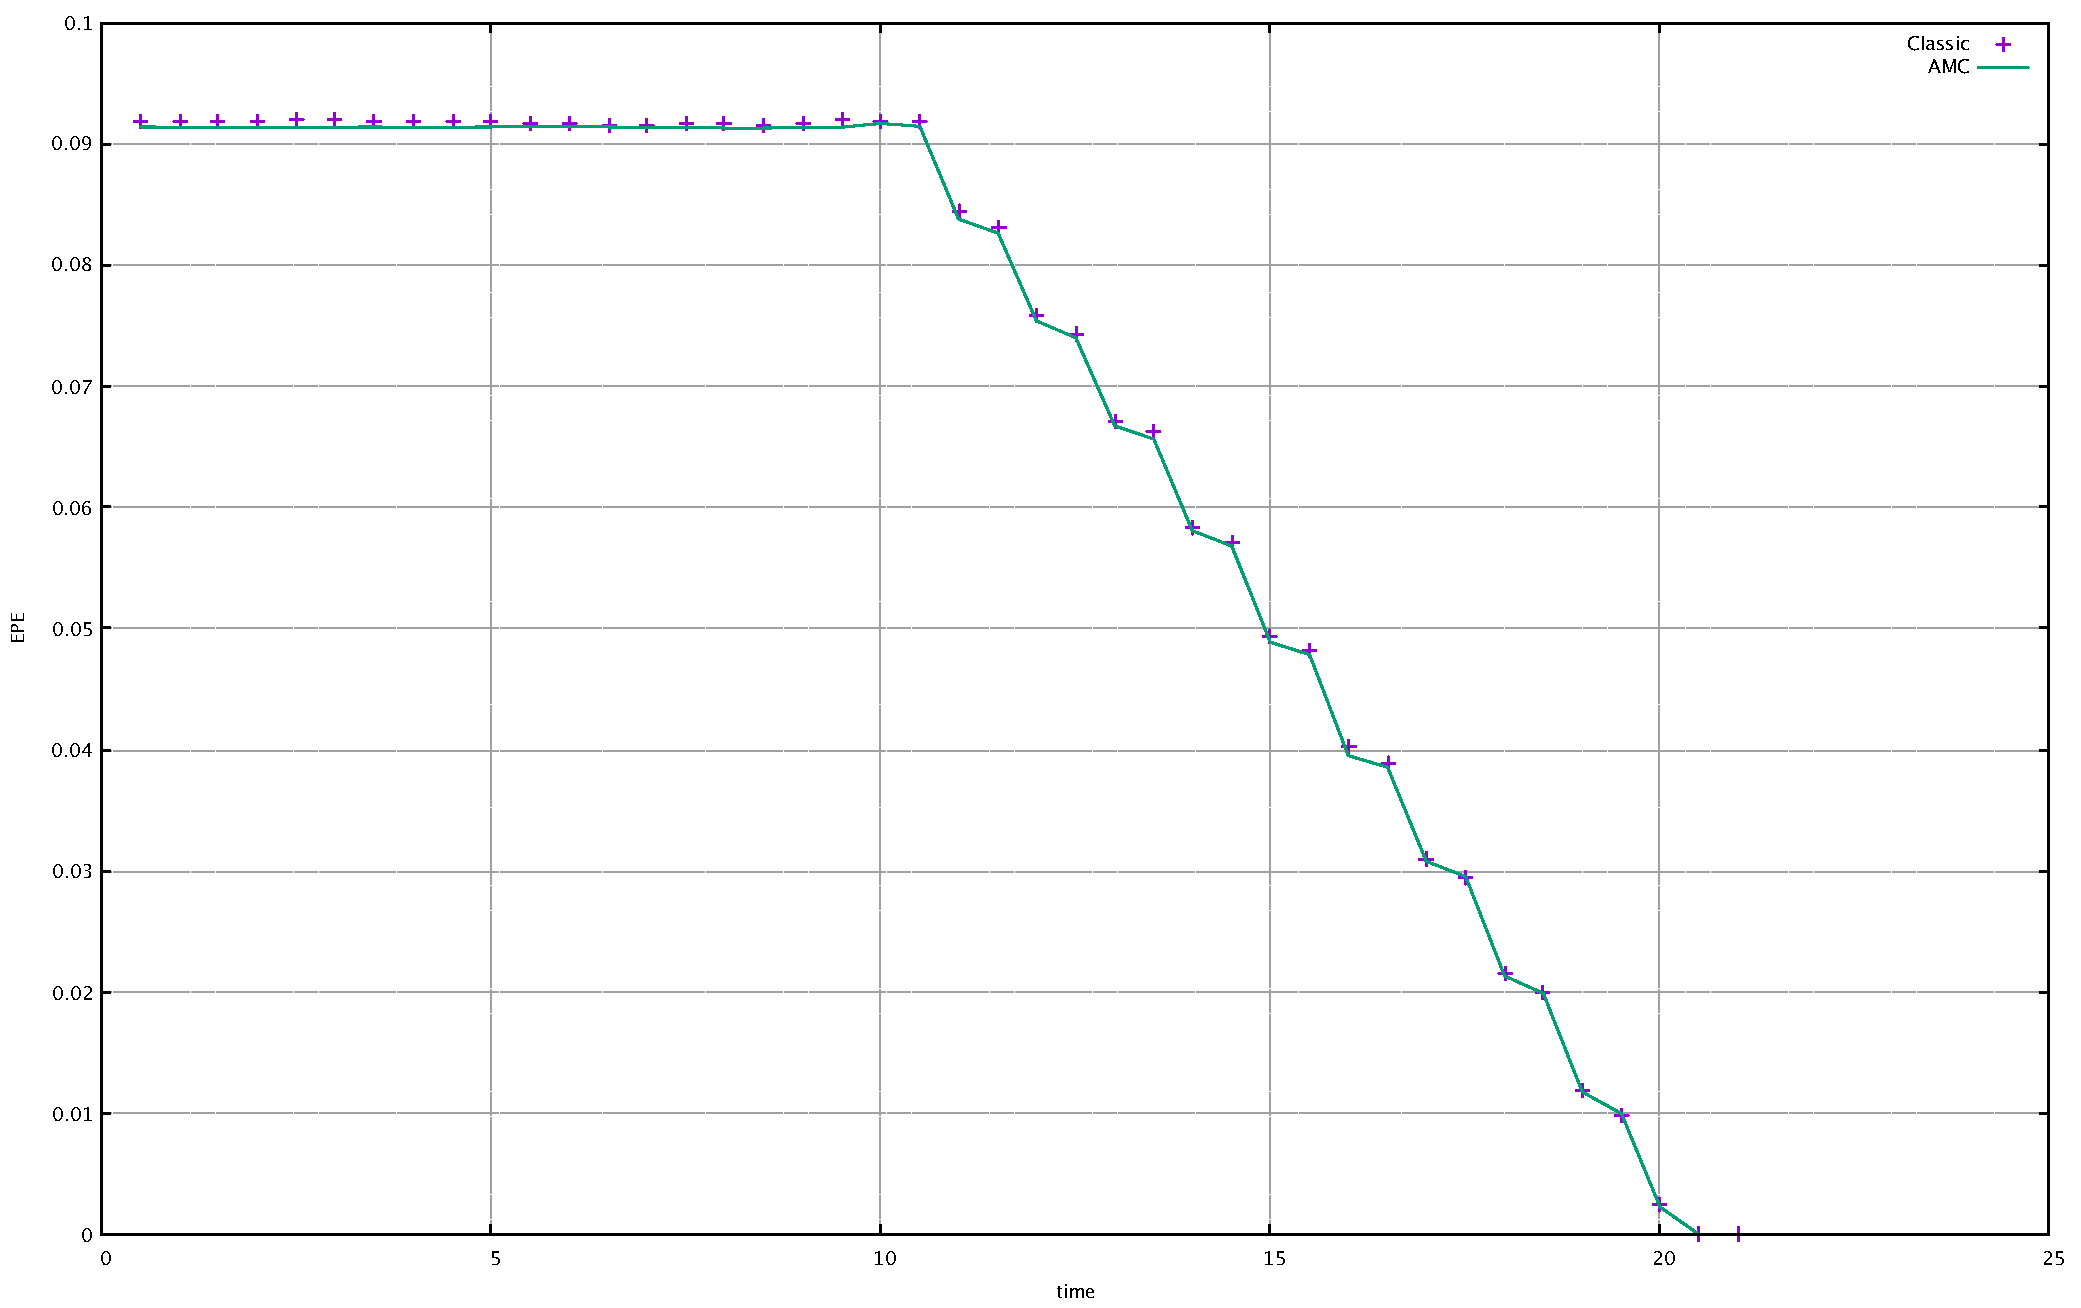
\includegraphics[width=0.8\textwidth]{epe_swaption.pdf}
  \caption{EPE of a EUR Bermudan Swaption computed with the classic and AMC valuation engines}
  \label{epe_swaption}
\end{figure}

\subsection{Single Currency Swap}

Figure \ref{epe_swap} shows the EPE and ENE for a 20y vanilla Swap in USD (taken from the AMC Example). The currency of
the amc calculator is USD in this case, i.e. it is different from the base ccy of the simulation (EUR). The consistency
of the classic and amc runs in particular demonstrates the correct application of the currency conversion factor
\ref{currency_conversion_factor}. To get a better accuracy for purposes of the plot in this document we increased the
number of training paths for this example to 50k and the order of the basis functions to 6.

\begin{figure}
  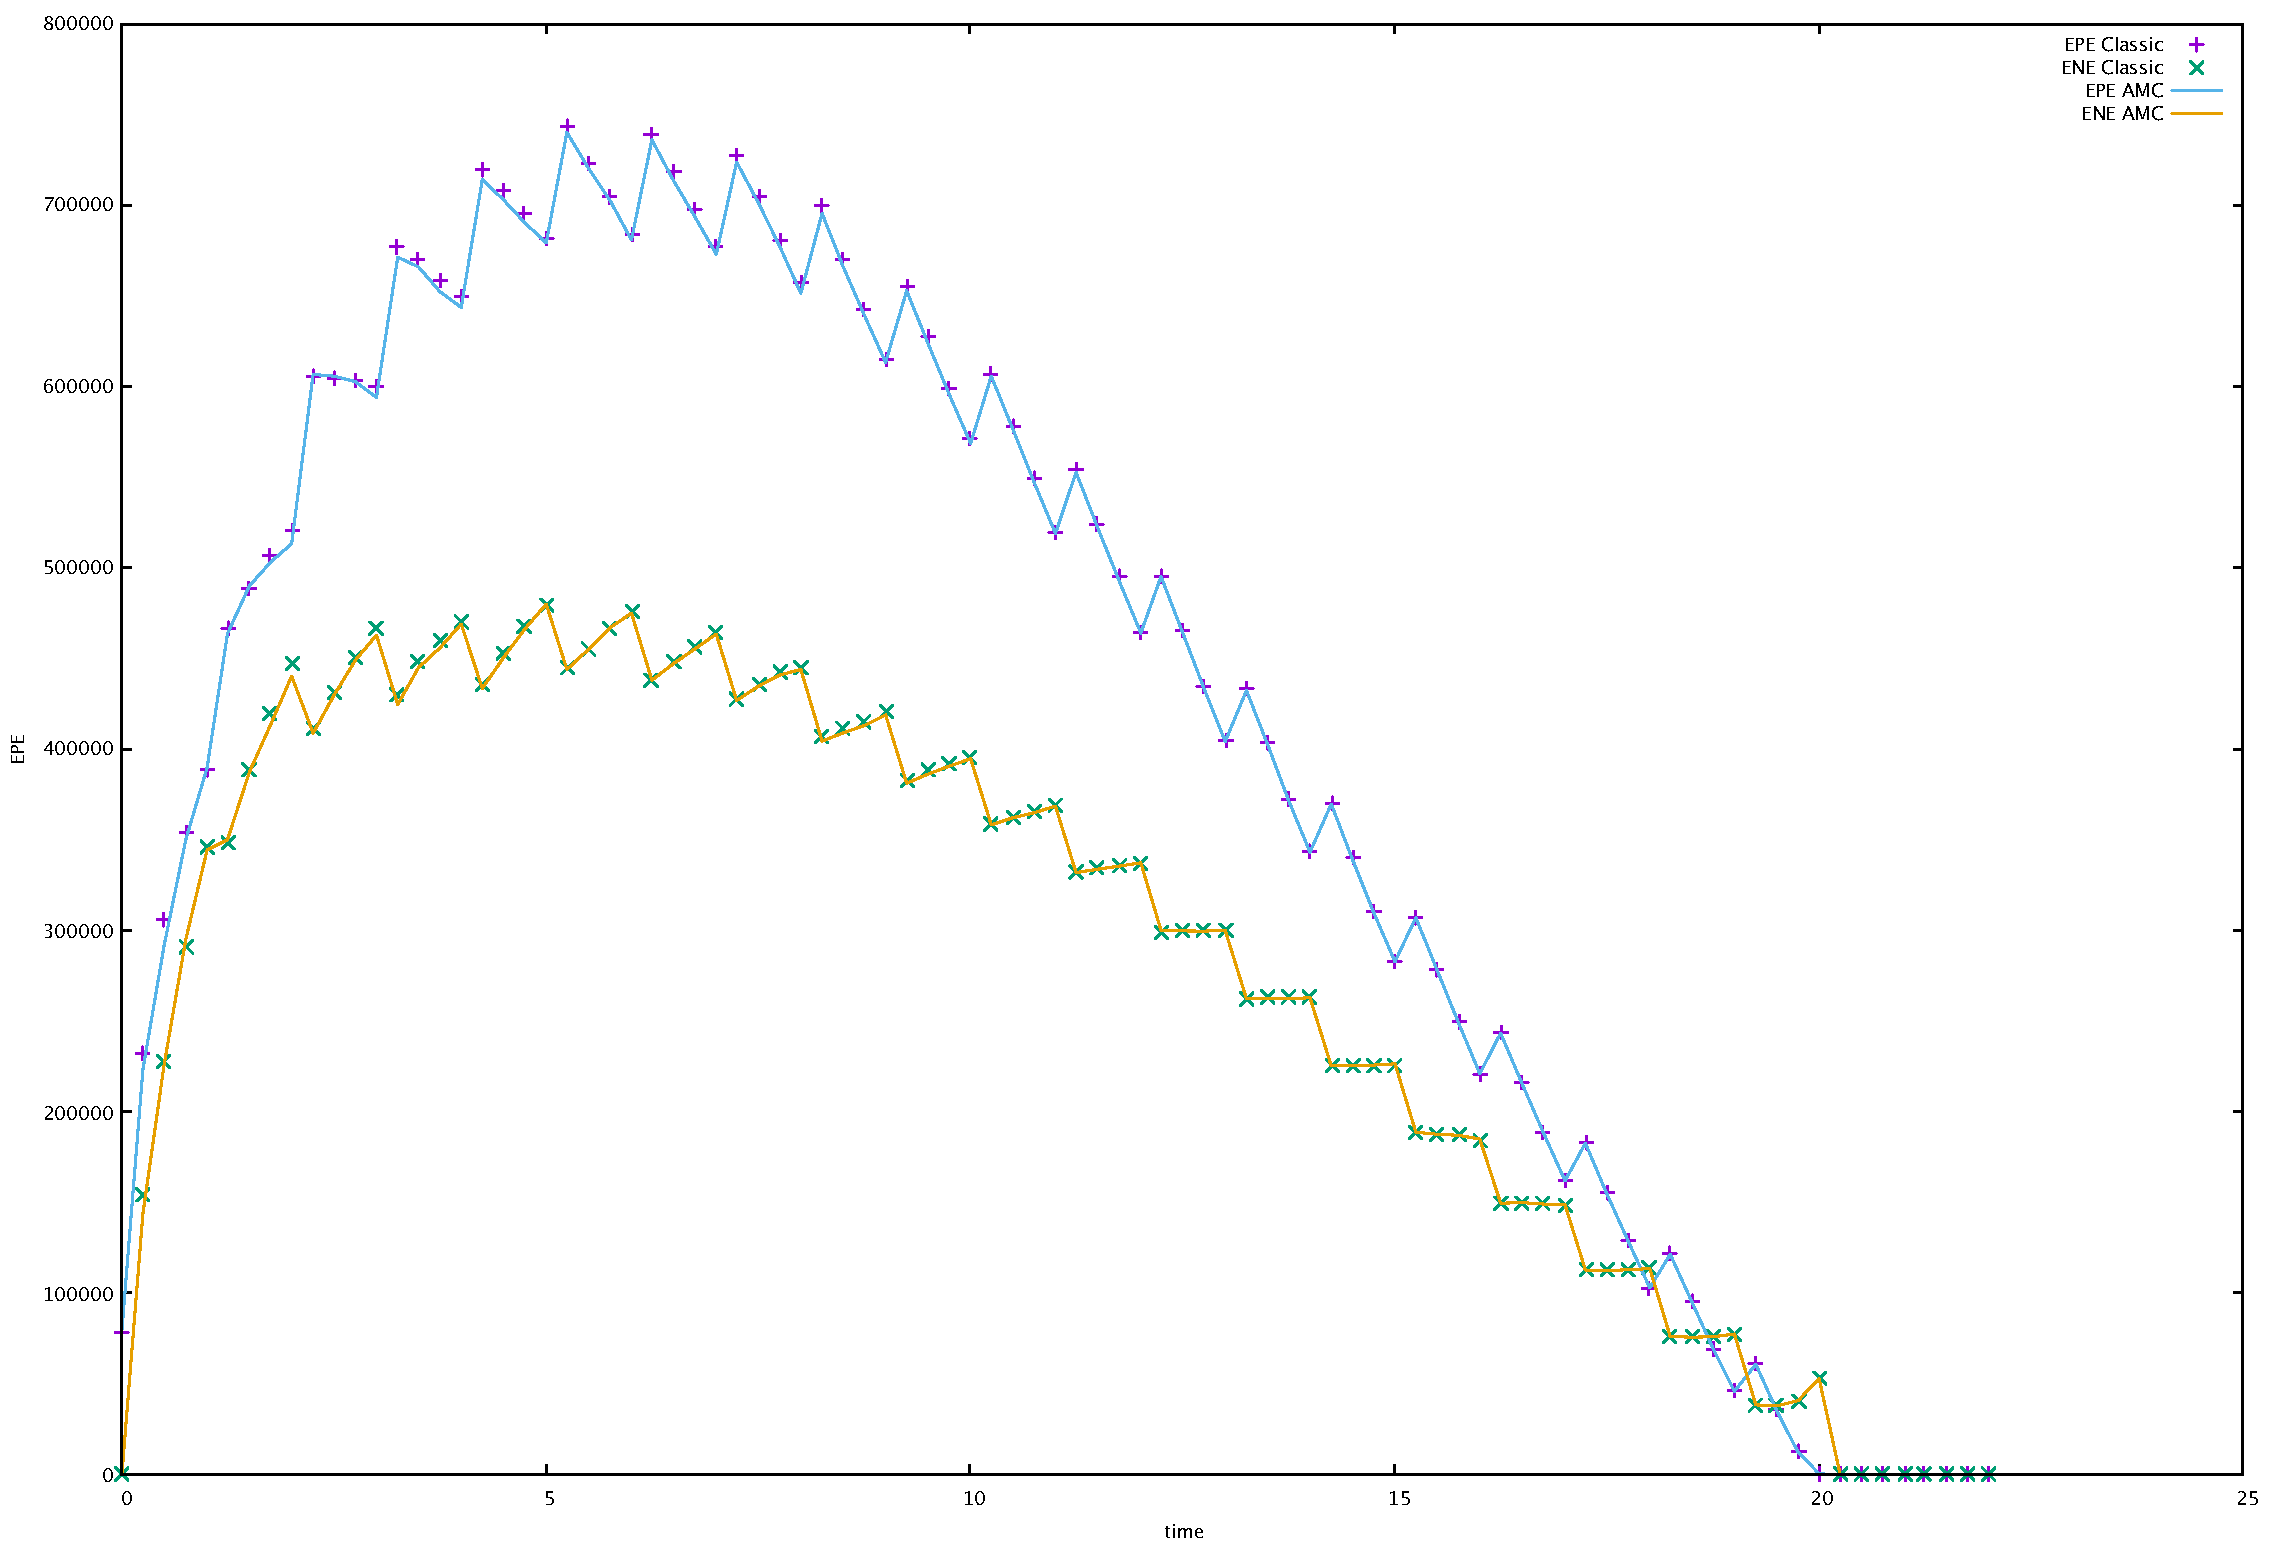
\includegraphics[width=0.8\textwidth]{epe_swap.pdf}
  \caption{EPE of a USD swap computed with the classic and AMC valuation engines}
  \label{epe_swap}
\end{figure}

\subsection{Cross Currency Swap}

Figure \ref{epe_ccyswap} shows the EPE and ENE for a 20y cross currency Swap EUR-USD (taken from the AMC Example). 

\begin{figure}
  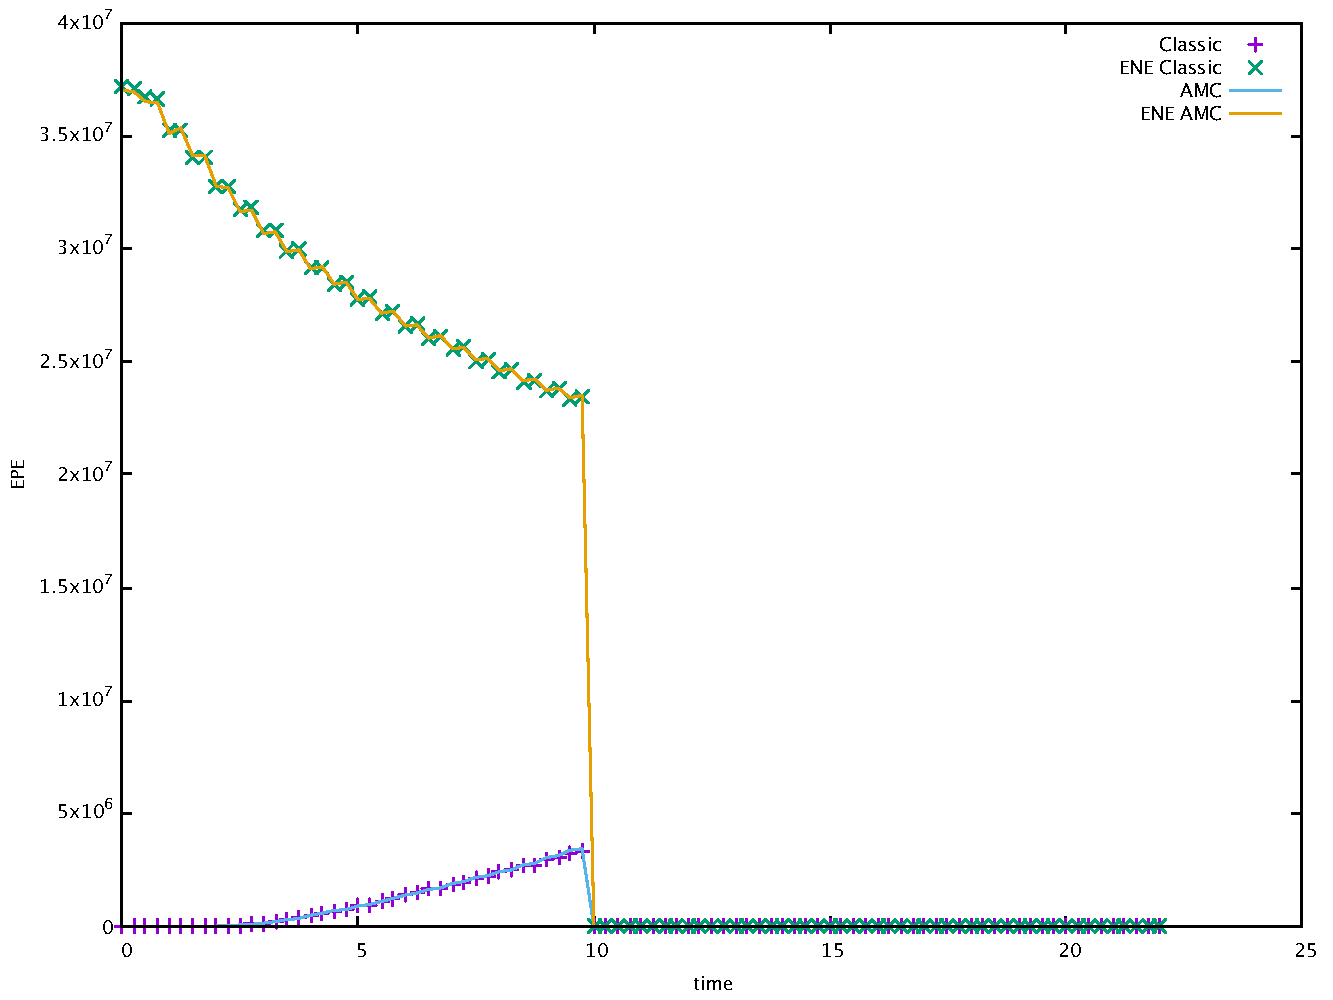
\includegraphics[width=0.8\textwidth]{epe_ccyswap.pdf}
  \caption{EPE of a EUR-USD cross currency swap computed with the classic and AMC valuation engines}
  \label{epe_ccyswap}
\end{figure}

\subsection{FX Option}

Figure \ref{epe_fxoption} shows the EPE and ENE for a vanilla FX Option EUR-USD with 10y1m expiry (taken from the AMC
Example). For the classic run the FX volatility surface is not implied by the cross asset model but kept flat, which
yields a slight hump in the profile. The AMC profile is flat on the other hand which demonstrates the consistency of the
FX Option pricing with the risk factor evolution model, see the discussion in \ref{overview}.

\begin{figure}
  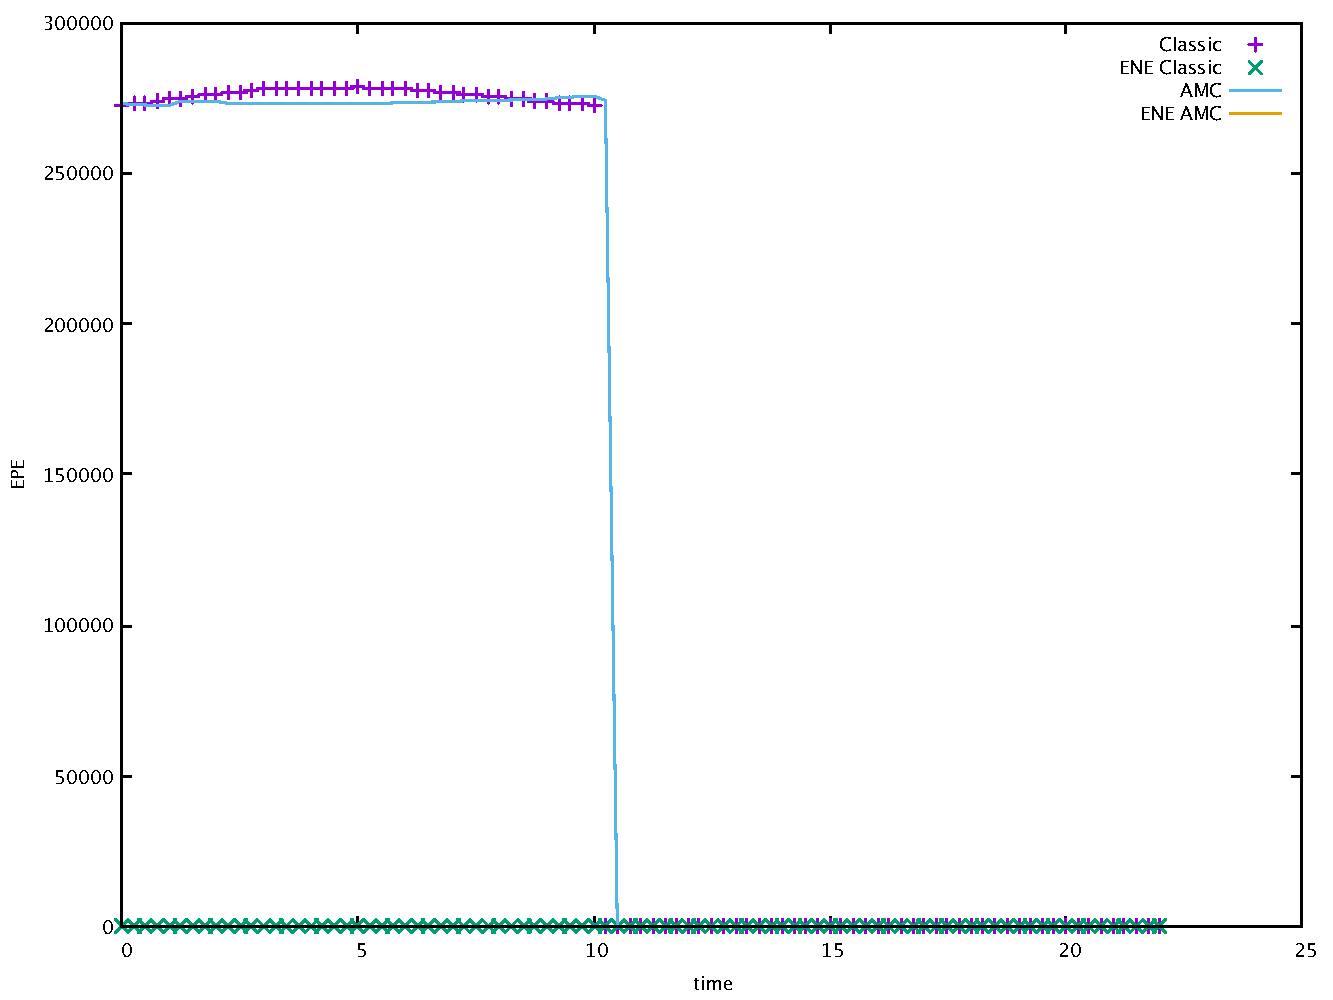
\includegraphics[width=0.8\textwidth]{epe_fxoption.pdf}
  \caption{EPE of a EUR-USD FX option computed with the classic and AMC valuation engines}
  \label{epe_fxoption}
\end{figure}

%==========================================
\section{Additional Features}\label{sec:side_products}
%==========================================

As a side product the AMC module provides plain MC pricing engines for Bermudan swaptions and a new trade type
\verb+MultiLegOption+ with a corresponding MC pricing engine.

\subsection{MC pricing engine for Bermudan swaptions}\label{sec:mc_bermudan_engine}

The following listing shows a sample configuration for the MC Bermudan swaption engine. The model parameters are
identical to the LGM Grid engine configuration. The engine parameters on the other hand are the same as for the AMC
engine, see \ref{sec:pricing_engine_config}.

\begin{minted}[fontsize=\footnotesize]{xml}
<Product type="BermudanSwaption">
  <Model>LGM</Model>
  <ModelParameters>
    <Parameter name="Calibration">Bootstrap</Parameter>
    <Parameter name="CalibrationStrategy">CoterminalDealStrike</Parameter>
    <Parameter name="Reversion_EUR">0.0050</Parameter>
    <Parameter name="Reversion_USD">0.0030</Parameter>
    <Parameter name="ReversionType">HullWhite</Parameter>
    <Parameter name="VolatilityType">HullWhite</Parameter>
    <Parameter name="Volatility">0.01</Parameter>
    <Parameter name="ShiftHorizon">0.5</Parameter>
    <Parameter name="Tolerance">1.0</Parameter>
  </ModelParameters>
  <Engine>MC</Engine>
  <EngineParameters>
    <Parameter name="Training.Sequence">MersenneTwisterAntithetic</Parameter>
    <Parameter name="Training.Seed">42</Parameter>
    <Parameter name="Training.Samples">10000</Parameter>
    <Parameter name="Training.BasisFunction">Monomial</Parameter>
    <Parameter name="Training.BasisFunctionOrder">6</Parameter>
    <Parameter name="Pricing.Sequence">SobolBrownianBridge</Parameter>
    <Parameter name="Pricing.Seed">17</Parameter>
    <Parameter name="Pricing.Samples">25000</Parameter>
    <Parameter name="BrownianBridgeOrdering">Steps</Parameter>
    <Parameter name="SobolDirectionIntegers">JoeKuoD7</Parameter>
  </EngineParameters>
</Product>
\end{minted}

\subsection{Multi Leg Options / MC pricing engine}

The following listing shows a sample MultiLegOption trade. It consists of

\begin{enumerate}
\item an option data block; this is optional, see below
\item a number of legs; in principle all leg types are supported, the number of legs is arbitrary and they can be in
  different currencies; if the payment currency of a leg is different from a floating index currency, this is
  interpreted as a quanto payoff
\end{enumerate}

If the option block is given, the trade represents a Bermudan swaption on the underlying legs. If the option block is
missing, the legs themselves represent the trade.

See \ref{sec:limitations_trade_features} and \ref{sec:limitations_recalibration} for limitations of the multileg option
pricing engine.

\begin{minted}[fontsize=\footnotesize]{xml}
<Trade id="Sample_MultiLegOption">
  <TradeType>MultiLegOption</TradeType>
  <Envelope>...</Envelope>
  <MultiLegOptionData>
    <OptionData>
      <LongShort>Long</LongShort>
      <OptionType>Call</OptionType>
      <Style>Bermudan</Style>
      <Settlement>Physical</Settlement>
      <PayOffAtExpiry>false</PayOffAtExpiry>
      <ExerciseDates>
        <ExerciseDate>2026-02-25</ExerciseDate>
        <ExerciseDate>2027-02-25</ExerciseDate>
        <ExerciseDate>2028-02-25</ExerciseDate>
      </ExerciseDates>
    </OptionData>
    <LegData>
      <LegType>Floating</LegType>
      <Payer>false</Payer>
      <Currency>USD</Currency>
      <Notionals>
        <Notional>100000000</Notional>
      </Notionals>
      ...
    </LegData>
    <LegData>
      <LegType>Floating</LegType>
      <Payer>true</Payer>
      <Currency>EUR</Currency>
      <Notionals>
        <Notional>100000000</Notional>
      </Notionals>
      ...
    </LegData>
  </MultiLegOptionData>
</Trade>
\end{minted}

The pricing engine configuration is similar to that of the MC Bermudan swaption engine, cf.
\ref{sec:mc_bermudan_engine}, also see the following listing.

\begin{minted}[fontsize=\footnotesize]{xml}
  <Product type="MultiLegOption">
  <Model>CrossAssetModel</Model>
  <ModelParameters>
    <Parameter name="Tolerance">0.0001</Parameter>
    <!-- IR -->
    <Parameter name="IrCalibration">Bootstrap</Parameter>
    <Parameter name="IrCalibrationStrategy">CoterminalATM</Parameter>
    <Parameter name="ShiftHorizon">1.0</Parameter>
    <Parameter name="IrReversion_EUR">0.0050</Parameter>
    <Parameter name="IrReversion_GBP">0.0070</Parameter>
    <Parameter name="IrReversion_USD">0.0080</Parameter>
    <Parameter name="IrReversion">0.0030</Parameter>
    <Parameter name="IrReversionType">HullWhite</Parameter>
    <Parameter name="IrVolatilityType">HullWhite</Parameter>
    <Parameter name="IrVolatility">0.0050</Parameter>
    <!-- FX -->
    <Parameter name="FxCalibration">Bootstrap</Parameter>
    <Parameter name="FxVolatility_EURUSD">0.10</Parameter>
    <Parameter name="FxVolatility">0.08</Parameter>
    <Parameter name="ExtrapolateFxVolatility_EURUSD">false</Parameter>
    <Parameter name="ExtrapolateFxVolatility">true</Parameter>
    <!-- Correlations IR-IR, IR-FX, FX-FX -->
    <Parameter name="Corr_IR:EUR_IR:GBP">0.80</Parameter>
    <Parameter name="Corr_IR:EUR_FX:GBPEUR">-0.50</Parameter>
    <Parameter name="Corr_IR:GBP_FX:GBPEUR">-0.15</Parameter>
  </ModelParameters>
  <Engine>MC</Engine>
  <EngineParameters>
    <Parameter name="Training.Sequence">MersenneTwisterAntithetic</Parameter>
    <Parameter name="Training.Seed">42</Parameter>
    <Parameter name="Training.Samples">10000</Parameter>
    <Parameter name="Pricing.Sequence">SobolBrownianBridge</Parameter>
    <Parameter name="Pricing.Seed">17</Parameter>
    <Parameter name="Pricing.Samples">25000</Parameter>
    <Parameter name="Training.BasisFunction">Monomial</Parameter>
    <Parameter name="Training.BasisFunctionOrder">4</Parameter>
    <Parameter name="BrownianBridgeOrdering">Steps</Parameter>
    <Parameter name="SobolDirectionIntegers">JoeKuoD7</Parameter>
  </EngineParameters>
</Product>
\end{minted}

Model Parameters special to that product are

\begin{enumerate}
\item \verb+IrCalibrationStrategy+ can be \verb+None+, \verb+CoterminalATM+, \verb+UnderlyingATM+
\item \verb+FXCalibration+ can be \verb+None+ or \verb+Bootstrap+
\item \verb+ExtrapolateFxVolatility+ can be \verb+true+ or \verb+false+; if false, no calibration instruments are used
  that require extrapolation of the market fx volatilty surface in option expiry direction
\item \verb+Corr_Key1_Key2+: These entries describe the cross asset model correlations to be used; the syntax for
  \verb+Key1+ and \verb+Key2+ is the same as in the simulation configuration for the cross asset model, see \cite{oreug}.
\end{enumerate}

%==========================================
\section{Implementation Details}\label{sec:implementation_details}
%==========================================

\subsection{AMC valuation engine and AMC pricing engines}

The \verb+AMCValuationEngine+ is responsible for generating a NPV cube for a portfolio of AMC enabled trades and
(optionally) to populate a \verb+AggregationScenarioData+ instance with simulation data for post processing, very
similar to the classic \verb+ValuationEngine+ in ORE.

The AMC valuation engine takes a cross asset model defining the risk factor evolution. This is set up identically to the
cross asset model used in the \\ \verb+CrossAssetModelScenarioGenerator+. Similarly the same parameters for the path
generation (given as a \verb+ScenarioGeneratorData+ instance) are used, so that it is guaranteed that both the AMC
engine and the classic engine produce the same paths, hence can be combined to a single cube for post processing. It is
checked, that a non-zero seed for the random number generation is used.

The portfolio that the AMC engine consumes is build against an engine factory set up by a pricing engine configuration
given in the amc analytics type (see \ref{sec:application_config}). This configuration should select special AMC engine
builders which (by a pure naming convention) have the engine type ``AMC''. These engine builders are retrieved from
\verb+getAmcEngineBuilders()+ in \verb+oreappplus.cpp+ and are special in that unlike usual engine builders they take
two parameters

\begin{enumerate}
\item the cross asset model which serves as a risk factor evolution model in the AMC valuation engine
\item the date grid used within the AMC valuation engine
\end{enumerate}

For technical reasons, the configuration also contains configurations for \\ \verb+CapFlooredIborLeg+ and \verb+CMS+
because those are used within the trade builders (more precisely the leg builders called from these) to build the
trade. The configuration can be the same as for T0 pricing for them, it is actually not used by the AMC pricing engines.

The AMC engine builders build a smaller version of the global cross asset model only containing the model components
required to price the specific trade. Note that no deal specific calibration of the model is performed.

The AMC pricing engines perform a T0 pricing and - as a side product - can be used as usual T0 pricing engines if a
corresponding engine builder is supplied, see \ref{sec:side_products}.

In addition the AMC pricing engines perform the necessary calculations to yield conditional NPVs on the given global
simulation grid. How these calcuations are performed is completely the responsibility of the pricing engines, altough
some common framework for many trade types is given by a base engine, see \ref{sec:amc_base_engine}. This way the
approximation of conditional NPVs on the simulation grid can be taylored to each product and also each single trade,
with regards to

\begin{enumerate}
\item the number of traning paths and the required date grid for the training (e.g. containing all relevant coupon and
  exercise event dates of a trade)
\item the order and type of regressoin basis functions to be used
\item the choice of the regressor (e.g. a TaRN might require a regressor augmented by the accumulated coupon amount)
\end{enumerate}

The AMC pricing engines then provide an additional result labelled \verb+amcCalculator+ which is a class implementing
the \verb+AmcCalculator+ interface which consists of two methods: The method \verb+simulatePath()+ takes a
\verb+MultiPath+ instance representing one simulated path from the global risk factor evolution model and returns an
array of conditional, deflated NPVs for this path. The method \verb+npvCurrency()+ returns the currency $c$ of the
calculated conditional NPVs. This currency can be different from the base currency $b$ of the global risk factor
evolution model. In this case the conditional NPVs are converted to the global base currency within the AMC valuation
engine by multiplying them with the conversion factor

\begin{equation}\label{currency_conversion_factor}
\frac{N_c(t) X_{c,b}(t)}{N_b(t)}
\end{equation}

where $t$ is the simulation time, $N_c(t)$ is the numeraire in currency $c$, $N_b(t)$ is the numeraire in currency
$b$ and $X_{c,b}(t)$ is the FX rate at time $t$ converting from $c$ to $b$.

The technical criterion for a trade to be processed within the AMC valuation is engine is that a) it can be built
against the AMC engine factory described above and b) it provides an additional result \verb+amcCalculator+. If a trade
does not meet these criteria it is simulated using the classic valuation engine. The logic that does this is located in
the overide of the method \verb+OREAppPlus::generateNPVCube()+.

The AMC valuation engine can also populate an aggregation scenario data instance. This is done only if necessary,
i.e. only if no classic simulation is performed anyway. The numeraire and fx spot values produced by the AMC valuation
engine are identical to the classic engine. Index fixings are close, but not identical, because the AMC engine used the
T0 curves for projection while the classic engine uses scenario simulation market curves, which are not exactly matching
those of the T0 market. In this sense the AMC valuation engine produces more precise values compared to the classic
engine.

\subsection{The multileg option AMC base engine and derived engines}\label{sec:amc_base_engine}

Table \ref{tbl:amcconfig} provides an overview of the implemented AMC engine builders. These builders use the following
QuantExt pricing engines

\begin{enumerate}
\item \verb+McLgmSwapEngine+ for single currency swaps
\item \verb+McCamCurrencySwapEngine+ for cross currency swaps
\item \verb+McCamFxOptionEngine+ for fx options
\item \verb+McLgmSwaptionEngine+ for Bermudan swaptions
\item \verb+McMultiLegOptionEngine+ for Multileg option
\end{enumerate}

All these engine are based on a common \verb+McMultiLegBaseEngine+ which does all the computations. For this each of the
engines sets up the following protected member variables (serving as parameters for the base engine) in their
\verb+calculate()+ method:

\begin{enumerate}
\item \verb+leg_+: a vector of \verb+QuantLib::Leg+
\item \verb+currency_+: a vector of \verb+QuantLib::Currency+ corresponding to the leg vector
\item \verb+payer_+: a vector of $+1.0$ or $-1.0$ double values indicating receiver or payer legs
\item \verb+exercise_+: a \verb+QuantLib::Exercise+ instance describing the exercise dates (may be \verb+nullptr+, if
  the underlying represents the deal already)
\item \verb+optionSettlement_+: a \verb+Settlement::Type+ value indicating whether the option is settled physically or
  in cash
\end{enumerate}

A call to \verb+McMultiLegBaseEngine::calculate()+ will set the result member variables

\begin{enumerate}
\item \verb+resultValue_+: T0 NPV in the base currency of the cross asset model passed to the pricing engine
\item \verb+underlyingValue_+: T0 NPV of the underlying (again in base ccy)
\item *\verb+amcCalculator_+: the AMC calculator engine to be used in the AMC valuation engine
\end{enumerate}

The specific engine implementations should convert the \verb+resultValue_+ to the npv currency of the trade (as defined
by the (ORE) trade builder) so that they can be used as regular pricing engine consistently within ORE. Note that only
the additional \verb+amcCalculator+ result is used by the AMC valuation engine, not any of the T0 NPVs directly.

%==========================================
\section{Limitations and Open Points}
%==========================================

This sections lists known limitations of the AMC simulation engine.

\subsection{Trade Features}\label{sec:limitations_trade_features}

Some trade features are not yet supported by the multileg option engine:

\begin{enumerate}
\item legs with fx resetting feature
\item legs with naked option = true
\item coupon types are restricted to Ibor and CMS
\item exercise flows (like a notional exchange common to cross currency swaptions) are not supported
\end{enumerate}

\subsection{Flows Generation (for DIM Analysis)}

At the current stage the AMC engine does not generate flows which are required for the DIM analysis in the post
processor.

\subsection{State interpolation for exercise decisions}

During the simulation phase exercise times of a specific trade are not necessarily part of the simulated time
grid. Therefore the model state required to take the exercise decision has in to be interpolated in general on the
simulated path. Currently this is done using a simple linear interpolation while from a pure methodology point of view a
Brownian Bridge would be preferable. In our tests we do not see a big impact of this approximation though.

\subsection{Missing recalibration of the MCMultiLegOptionEngine}\label{sec:limitations_recalibration}

The MC Multi Leg Option Engine builder uses the \verb+CrossAssetModelBuilder+ to set up the pricing model. This class
does not implement the \verb+ModelBuidler+ interface meaning that the model is not recalibrated in a sensitivity
analysis run. Therefore the sensitivities calculated by this engine are not valid.

\subsection{Basis Function Selection}

Currently the basis function system is generated by specifying the type of the functions and the order, see
\ref{sec:pricing_engine_config}. The number of indenpendent variables varies by product type and details. Depending on
the number of independent variables and the order the number of generated basis functions can get quite big which slows
down the computation of regression coefficients. It would be desirable to have the option to filter the full set of
basis functions, e.g. by explicitly enumerating them in the configuration, so that a high order can be chosen even for
products with a relatively large number of independent variables (like e.g. FX Options or Cross Currency Swaps).

%==========================================
\section{Outlook}
%==========================================

\subsection{Trade Compression}

For vanilla trades where the regression is only required to produce the NPV cube entries (and not to take exercise
decisions etc.) it is not strictly necessary to do the regression analysis on a single trade level\footnote{except
  single trade exposures are explicitly required of course}. Although in the current implementation there is no direct
way to do the regression analysis on whole (sub-)portfolios instead of single trades, one can represent such a
subportfolio as a single technical trade (e.g. as a single swap or multileg option trade) to achieve a similar
result. This might lead to better performance than the usual single trade calculation. However one should also try to
keep the regressions as low-dimensional as possible (for performance and accuracy reasons) and therefore define the
subportfolios by e.g. currency, i.e. as big as possible while at the same time keeping the associated model dimension as
small as possible.

%==========================================
% \begin{appendix}
%==========================================
% \end{appendix}

%\addcontentsline{toc}{section}{Appendices}

\begin{thebibliography}{1}

\bibitem{oreug} ORE User Guide, \url{http://www.opensourcerisk.org/documentation/}

\end{thebibliography}

\end{document}
